\documentclass[11pt, aspectratio=169, compress]{beamer}
\usetheme[progressbar=frame title, numbering=fraction]{metropolis}      % Use metropolis theme 
\setbeamertemplate{section in toc}[sections numbered]
\setbeamertemplate{subsection in toc}[subsections numbered]
\useoutertheme[subsection=false]{miniframes}
\setbeamercolor{section in head/foot}{fg=white, bg=mDarkTeal}
\setbeamercolor{background canvas}{bg=white}
\setbeamerfont{section in head/foot}{series=\bfseries}

\usefonttheme[onlymath]{serif}
\usepackage{amsmath}
\usepackage{remreset}
\usepackage{ragged2e}
\usepackage{booktabs}
\usepackage{makecell}
\usepackage{float}
\usepackage{subfig}
\usepackage{tikz}
\usetikzlibrary{positioning,calc}
\usepackage[flushleft]{threeparttable}	% 3 part table 
\usepackage[justification=centering]{caption}
\captionsetup{skip=0pt}
\graphicspath{{./fig/}}

\makeatletter
\let\beamer@writeslidentry@miniframeson=\beamer@writeslidentry
\def\beamer@writeslidentry@miniframesoff{%
	\expandafter\beamer@ifempty\expandafter{\beamer@framestartpage}{}% does not happen normally
	{%else
		% removed \addtocontents commands
		\clearpage\beamer@notesactions%
	}
}
\newcommand*{\miniframeson}{\let\beamer@writeslidentry=\beamer@writeslidentry@miniframeson}
\newcommand*{\miniframesoff}{\let\beamer@writeslidentry=\beamer@writeslidentry@miniframesoff}
\beamer@compresstrue
\makeatother

%==============================================================
% Title Page
%==============================================================
%Information to be included in the title page:
\title{Programación 101}
\author{Rony Rodriguez-Ramírez} 
\institute{The World Bank | DIME \\ LAMBDA}
\titlegraphic{\hfill
\includegraphics[height=1.5cm]{dime}}
\date{\today}
%==============================================================
\begin{document}
	
\begin{frame}[plain]
	\maketitle 
\end{frame}

%------------------------------------------------
\section{Introducción al Curso}
%-----------------------------------------------
\subsection{Introducción al Curso}
%-----------------------------------------------
\begin{frame}{Introducción}
	¿Quién soy? 
	\begin{itemize}
		\item Nombre: Rony Rodrigo Maximiliano Rodríguez-Ramírez
		\item Trabajo: Banco Mundial, Washington, D.C.  
		\begin{itemize}
			\item Development Impact Evaluation Unit (DIME)
		\end{itemize}
		\item Educación: Economista con máster en Development Policy (KDI School)
		\item Experiencia: 
		\begin{itemize}
			\item Innovations for Poverty Action (IPA) -- Instituto Tecnológico Autónomo de México
			\item Monash University (Australia)
			\item KDI School of Public Policy and Management
		\end{itemize} 
		\item La mayoría de mi trabajo es evaluación de impacto de Randomized Controlled Trials en países en desarrollo (e.g., Rwanda, Liberia, etc.).
	\end{itemize}
\end{frame}
%-----------------------------------------------
\section{Organización del Curso}
%-----------------------------------------------
\subsection{Organización del Curso}
%-----------------------------------------------
\begin{frame}{Enfoque del Curso}
	\begin{itemize}
		\item ¿Por qué es importante aprender un software de análisis econométrico hoy en día (Stata, R, etc.)? 
		\item Mejoramiento del conocimiento de programación aplicada a la econometría y la investigación.
		\item Buenas prácticas de programación de la Unidad de Evaluación de Impacto (DIME) del Banco Mundial.
	\end{itemize}
\end{frame}
%-----------------------------------------------
\begin{frame}{Objetivos}
	\textbf{Objetivos del Curso:} 
	\begin{itemize}
		\item Aprender los conceptos clave y las técnicas econométricas asociadas a la programación estadísticas usando Stata enfatizando la eficiencia de escribir códigos: 
		\begin{itemize}
			\item Desarrollar buenos hábitos de programación.
			\item Aprende a implementar programación básica y avanzada.
			\item Aprenda varias características y detalles específicos del lenguaje de programación popular en econometría, Stata.
		\end{itemize}

	\end{itemize}
\end{frame}
%-----------------------------------------------
\begin{frame}{Sesiones}
	Este curso estará dividio en 5 tópicos fundamentales: 
	\begin{enumerate}
		\item Programación 101 (2 horas)
		\item Manejo y Limpieza de Datos (2 horas)
		\item Construcción de Datos (2 horas)
		\item Análisis de Datos (4 horas)
		\item Programando modelos de evaluación de Impacto
		\begin{enumerate}
			\item RCTs y Datos Panel (2 horas)
			\item Diferencias en Diferencias (2 horas)
			\item Regresión Discontinua (2 horas)
		\end{enumerate}
	\end{enumerate}	
\end{frame}
%-----------------------------------------------

%-----------------------------------------------
\section{Materiales del Curso}
%-----------------------------------------------
\subsection{Materiales del Curso}
%-----------------------------------------------
\begin{frame}{Repositorio en Github}
	Los materiales del curso se pueden encontrar en el siguiente \href{https://github.com/lambda-stata/course-materials}{\color{blue}{enlace}}. Este repositorio será actualizado semalmente con las siguietes carpetas. A su vez, subiré la misma información al \href{https://aulavirtual.grupolambda.com.pe/index/curso/id/5427}{\color{blue}{Aula Virtual}}. 
	\begin{enumerate}
		\item lectures (Slides)
		\begin{itemize}
			\item 01-programming-intro
			\item 02-manejo-limpieza-datos
		\end{itemize}
		\item data
		\item codes (Stata)
		\begin{itemize}
			\item 01-programming-intro
			\item 02-manejo-limpieza-datos
		\end{itemize} 
		\item syllabus
	\end{enumerate}
\end{frame}
%-----------------------------------------------
\begin{frame}{Encuestas}
	\begin{itemize}
		\item Uso de Stata
		\item Uso de Git
		\item Uso de \LaTeX
	\end{itemize}
\end{frame}
%-----------------------------------------------
%-----------------------------------------------
\section{Programación 101}
%-----------------------------------------------
\subsection{Programación 101}
%-----------------------------------------------
\begin{frame}{Excel vs Stata}
	¿Puedo ocupar Excel para análisis de regresiones?
\end{frame}
%-----------------------------------------------
\begin{frame}{La principal razón por la cual escribimos códigos}
	\begin{itemize}
		\item En Excel, se realiza cambios directamente en los datos y guarda nuevas versiones del conjunto de datos. 
		\item En Stata (o R), realiza cambios en las instrucciones sobre cómo pasar de los datos sin procesar al análisis final y guarda nuevas versiones de las instrucciones.
		\begin{itemize}
			\item En Stata utilizamos do files (or ado files).
			\item En R utilizamos RScripts.
		\end{itemize}
	\end{itemize}
\end{frame}
%-----------------------------------------------
\begin{frame}{Tu código es un resultado}
	\begin{block}{¿Cómo deberíamos de tratar nuestro código?}
		Los investigadores a menudo tratan el código como un medio para un fin, pero el punto principal de esta presentación es que su código es tanto un fin en sí mismo como el documento o el informe que está escribiendo.
	\end{block}
\end{frame}
%-----------------------------------------------
\begin{frame}{Objetivo de esta primera sesión}
	\begin{itemize}
		\item Para convertirse en un gran coder, ambos deben codificar como un coder y pensar como un coder.

		\item Ambos requieren mucha práctica para dominar, pero el objetivo de esta sesión es brindarle un marco para pensar como un codificador respondiendo preguntas como:
		
		\begin{itemize}
			\item ¿Por qué programar?
		
			\item ¿Cómo programo para que sea lo más útil para otras personas de mi equipo?
		\end{itemize}	
	\end{itemize}

\end{frame}
%-----------------------------------------------
\begin{frame}{Programar en academia vs workplace}
	\begin{itemize}
		\item En academia: 
		\begin{itemize}
			\item Estar en el correcto importa. 
		\end{itemize}
		\item Workplace:
		\begin{itemize}
			\item Estar en lo correcto es igual de importante que en la academia,
			\item Los miembros del equipo pasados, actuales y futuros contribuirán al mismo código y, por lo tanto, debemos estandarizar cómo programamos y centrarnos en las habilidades para programar como equipo.
		\end{itemize}
	\end{itemize}	
\end{frame}
%-----------------------------------------------
\begin{frame}{Pensamiento crítico sobre los datos.}
	\begin{itemize}
		\item ¿Creo en este número?
		\item ¿Qué puede salir mal en mi código?
		\item ¿Cómo se tratarán los valores perdidos en este comando?
		\item ¿Qué pasaría si se agregaran más observaciones al conjunto de datos?
		\item ¿Qué sucedería si algunas observaciones se eliminaran del conjunto de datos?
	\end{itemize}
\end{frame}
%-----------------------------------------------
\subsection{Manejo de los datos}
%-----------------------------------------------
\begin{frame}{Explore un conjunto de datos sin procesar}
	¿Qué es lo primero que buscamos cada vez que abre un nuevo conjunto de datos por primera vez?

	\begin{enumerate}
		\item Unidad de observación.
		\item Identificación completa y única de una variable ID. 
	\end{enumerate}
\end{frame}
%-----------------------------------------------
\begin{frame}{Explore a raw data set}
	\begin{itemize}
		\item Household\_data.csv
	\end{itemize}
	\begin{figure}[H]
		\centering
		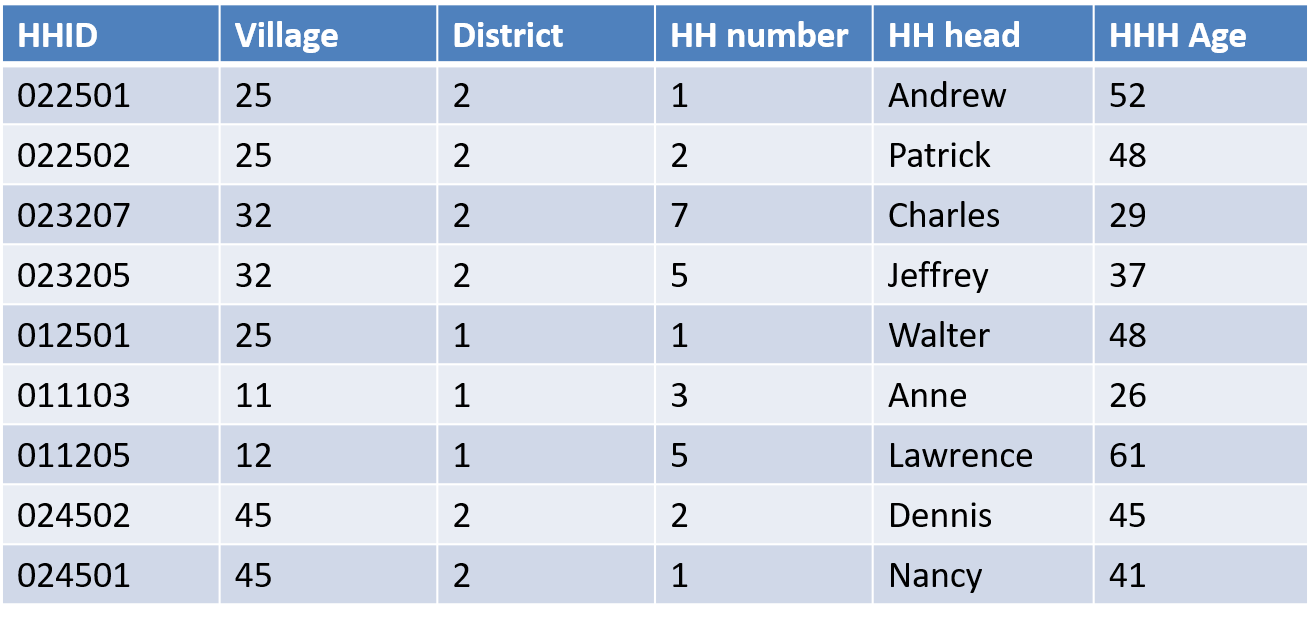
\includegraphics[width=0.8\textwidth]{hh_data.png}
	\end{figure}
\end{frame}
%-----------------------------------------------
\begin{frame}{Explore a raw data set}
	\begin{itemize}
		\item Clinic\_data.csv
	\end{itemize}
	\begin{figure}[H]
		\centering
		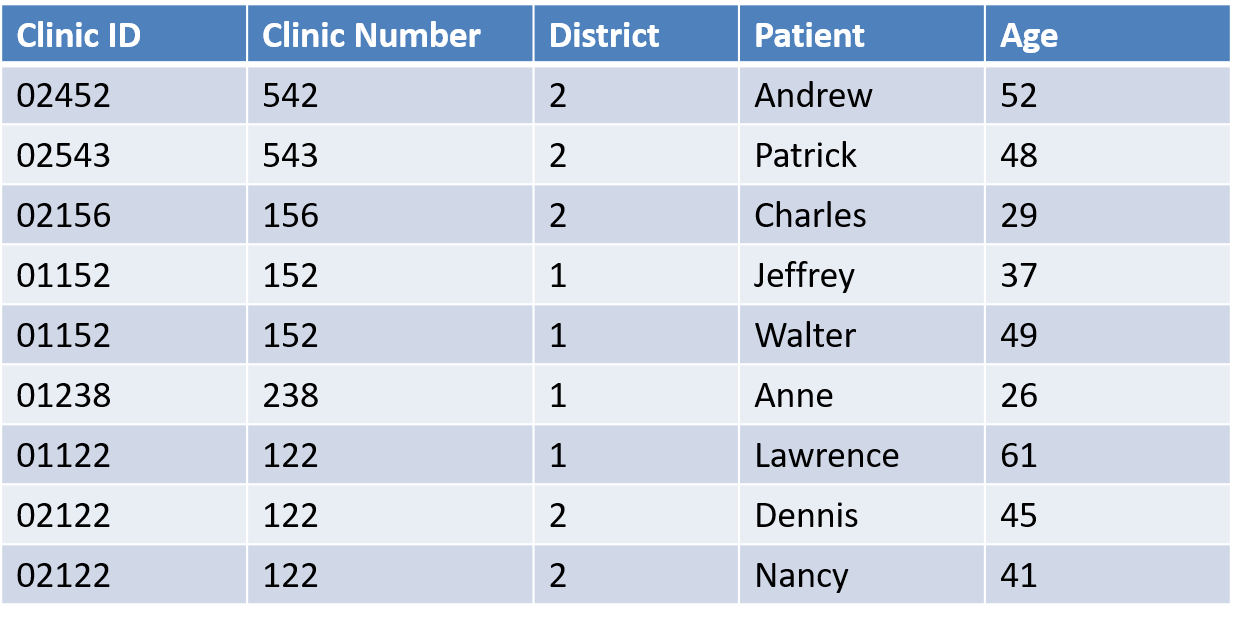
\includegraphics[width=0.8\textwidth]{clinic_data.png}
	\end{figure}
\end{frame}
%-----------------------------------------------
\begin{frame}{Variable ID}
	\begin{itemize}
		\item Solo trabaje con un conjunto de datos que tenga una variable de ID. Si el conjunto de datos que ha recibido no tiene uno, entonces crearlo es su primera tarea.
		\item Probar que la variable ID es única y completamente identificable.
		\item Use solo una variable como variable de ID.
	\end{itemize}
\end{frame}
%-----------------------------------------------
\begin{frame}{División de roles en el trabajo de datos}
	\textbf{Asistentes de investigación}
	\begin{itemize}
		\item Nadie mirará los datos tanto como el RA.
		\item Las irregularidades en los datos que la RA no identifica a menudo nunca se descubrirán
	\end{itemize}
	\textbf{Economistas}
	\begin{itemize}
		\item A cargo de decidir qué irregularidades se corregirán y cómo.
		\item Los economistas dependen completamente de los RA para identificar irregularidades y obtener la información para tomar la mejor decisión.
	\end{itemize}
\end{frame}
%-----------------------------------------------
\subsection{Coding Styles}
%-----------------------------------------------
\begin{frame}{Estilo}
	Stata no distingue entre un espacio vacío y muchos espacios vacíos, o un salto de línea o muchos saltos de línea. Es una gran diferencia para el ojo humano y nunca compartiríamos un documento de Word, una hoja de Excel o una presentación de PowerPoint sin pensar en espacios en blanco, aunque en este caso lo llamamos formato.

	\begin{center}
		¿Es esta diapositiva fácil de leer?
	\end{center}
\end{frame}
%-----------------------------------------------
\begin{frame}{White space - Espacio blanco}
	\begin{itemize}
		\item Stata no distingue entre un espacio vacío y muchos espacios vacíos, o un salto de línea o muchos saltos de línea.

		\item Es una gran diferencia para el ojo humano y nunca compartiríamos un documento de Word, una hoja de Excel o una presentación de PowerPoint sin pensar en espacios en blanco, aunque en este caso lo llamamos formato.
	\end{itemize}
\end{frame}
%-----------------------------------------------
\begin{frame}{Líneas verticales}
	\begin{figure}[H]
		\centering
		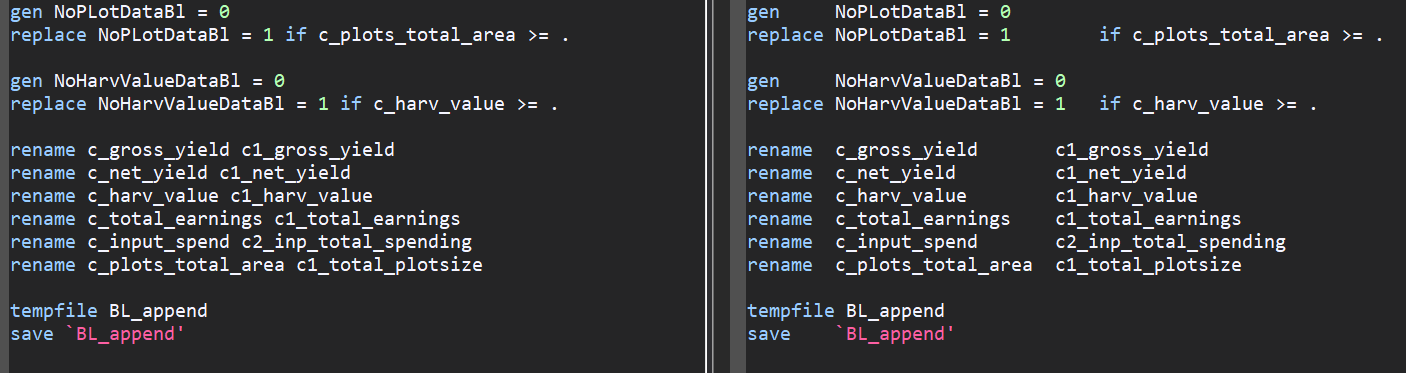
\includegraphics[width=1\textwidth]{code_vertical.png}
	\end{figure}
\end{frame}
%-----------------------------------------------
\begin{frame}{Líneas verticales}
	\begin{figure}[H]
		\centering
		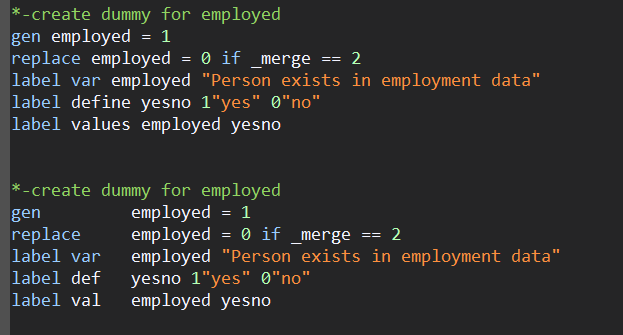
\includegraphics[width=0.8\textwidth]{code_vertical2.png}
	\end{figure}
\end{frame}
%-----------------------------------------------
\subsection{Documentación}
%-----------------------------------------------
\begin{frame}{Uso del archivos de ayuda y el conocimiento de programación}
	\begin{figure}[H]
		\centering
		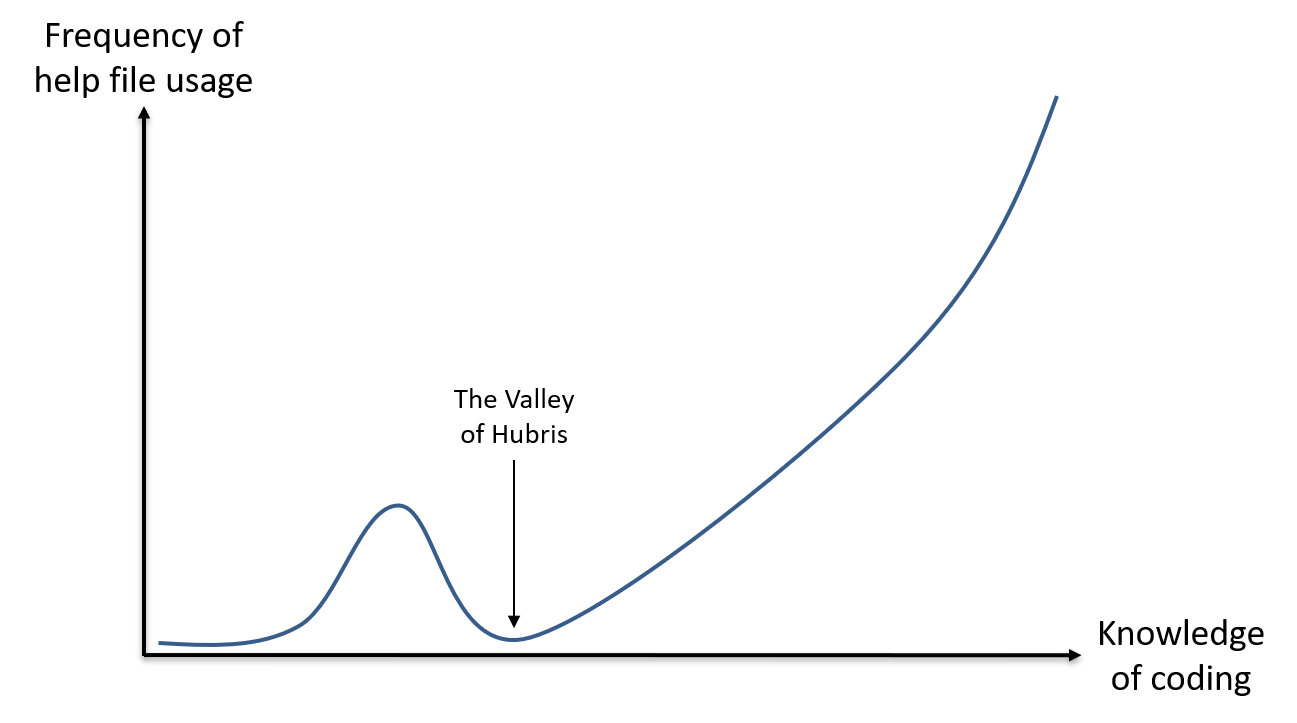
\includegraphics[width=0.8\textwidth]{dunning.png}
	\end{figure}	
\end{frame}
%-----------------------------------------------
\begin{frame}{Archivos de ayuda (help files)}
	\begin{itemize}
		\item Escriba Stata: \texttt{help nombre\_comando} 
		\item ¡Acostúmbrate a usar el archivo de ayuda con la mayor frecuencia posible!
		\begin{itemize}
			\item Incluso con comandos familiares, siempre más para aprender.
		\end{itemize}
		\item Los archivos de ayuda son solo resúmenes del manual de referencia prácticas de codificación, errores comunes, enfoques alternativos.
	\end{itemize}
\end{frame}
%-----------------------------------------------
\subsection{¿Cómo mejorar en programación}
%-----------------------------------------------
\begin{frame}{¿Dónde están las regresiones}
	\begin{itemize}
		\item Todavía no hemos realizado nada sobre regresiones. 
		\item En programación, el análisis es la parte fácil siempre que el conjunto de datos esté configurado correctamente para el análisis.
		\item Cómo usar los comandos para el análisis es mucho más fácil buscarlo en Google o preguntarle a alguien cómo hacerlo comparado con  la limpieza de datos, la gestión de datos y el aseguramiento de la calidad de los datos.
	\end{itemize}
\end{frame}
%-----------------------------------------------
\begin{frame}{En palabras sencillas}
	\begin{center}
		``Cuando tu código funciona, solo estás a medias''. 
	\end{center}
\end{frame}
%-----------------------------------------------
\begin{frame}{Revisar el código de las demás}
	\begin{itemize}
		\item Compare su código y discuta las diferencias con otras personas.
		\item Pregunte qué es más fácil de entender si piensa en su \texttt{do file} como una instrucción. ¿Que es difícil?
		\item Aplique un pensamiento crítico al trabajo de datos al código de cada uno, i.e., pruebe si habrá errores en su código, o si faltan datos.
		\item Si nadie le permite ver su código, pídale a las personas que lo vean. 
		\begin{itemize}
			\item ¿Alguna vez le has pedido a alguien que te ayude a corregir tu documento de Word?
		\end{itemize}
	\end{itemize}
\end{frame}
%-----------------------------------------------
\begin{frame}{Leer el código de otras personas}
	\begin{itemize}
		\item Busque el código en GitHub
		\item \href{https://github.com/trending/stata}{https://github.com/trending/stata} (Stata)
		\item \href{https://github.com/vikjam/mostly-harmless-replication}{https://github.com/vikjam/mostly-harmless-replication} (Stata y otros idiomas)
		\item Googlear, pero antes, hágase preguntas críticas sobre el código que encontró.
		\item ¿Por qué esta persona programó de esta manera?
		\item ¿Esto se aplica a mi contexto?
	\end{itemize}	
\end{frame}
%-----------------------------------------------
\begin{frame}{Literatura de gestión de bases de datos}
	\begin{itemize}
		\item La carpeta de su proyecto es una base de datos informal, y personas muy inteligentes que trabajan con bases de datos han estado pensando mucho en esto.
		\item No tengo un libro específico para recomendar, ya que no conozco un libro escrito para nuestro contexto, por lo que este método no es para los débiles
	\end{itemize}		
\end{frame}
%-----------------------------------------------
\begin{frame}{Conclusión}
	\begin{itemize}
		\item Su código es una herramienta que debe desarrollar como si otras personas lo estuvieran usando.

		\item Solicite ayuda de sus pares para revisar su código.
		
		\item Al enviar el código, formatee con el mismo cuidado que formatearía su currículum o su carta de presentación.
	\end{itemize}
\end{frame}
%==============================================================
% END
%==============================================================
\miniframesoff 	
\begin{frame}[plain, standout]
Nos vemos mañana.
\end{frame}
%------------------------------------------------
\end{document}		
